\section{Kinetic Monte Carlo Setup}
\label{Chap:Al/Vac:section:KMC}


The \ac{kMC} code was written in C++17\cite{Zhang2020KNN2}. Our code has two dependent libraries. First, we used an open-source C++ module called ``keras2cpp'' to read the Keras model trained in python\cite{Perevozchikov2019}. Second, we also applied another open-source numerical library, called Armadillo\cite{sanderson2016armadillo, sanderson2018user}, to do matrix multiplication for rotating current configurations to symmetry equivalent ones. As we mentioned above, all four symmetry equivalent structures needed to be calculated to evaluate vacancy migration barriers accurately, and both forward and backward vacancy migration barriers were required. Therefore, a total of 8 calculations were needed for one event. Therefore it becomes important to speed up calculations. We used \ac{MPI} to parallelize our \ac{kMC} simulations. Two parts are benefited significantly from parallelism implementation: 1) building initial neighbor list of every atom; 2) \ac{kMC} event rate calculations. Note that once the initial neighbor list is built, one can keep updating the neighbor list on the fly. Besides, vacancy migration barriers and event rates of 12 possible jumping events of one vacancy were distributed to different cores and collected afterward. We tested the scalability of the code, as shown in Figure \ref{Chap:Al/Vac:fig:scale}. A (30$\times$30$\times$30) supercell containing 108,000 atoms, was used for this testing. Calculations up to 80,000-steps were tested and benchmarked with the usage of different numbers of nodes. For very limited-steps cases, such as 10,000 steps, more cores showed more advantages, as the initial setup of the neighbor list takes a considerable amount of time. As the simulation goes on, the cost of communication between cores does not affect the scalability significantly.


\subsection{\acf{kMC} Algorithm}
Most parts of the \ac{kMC} algorithm were implemented following the approach we discussed in Algorithm \ref{algo:kMC} of Chapter \ref{chap:meth:KMC}. In this implementation, several points are worth noticing: 1) Event list is determined on the fly. We consider the first nearest neighbor exchange of vacancies. This yields a total of 12 times the total number of vacancies possible events. 2) Then, a \ac{NN} potential is used, instead of traditional empirical potentials or analytical equations, to evaluate vacancy migration barriers. Noting that all the four symmetry equivalent structures are taken into consideration. 3) At each step, both the forward and backward vacancy migration barriers of executing the current jump are calculated to obtain the energy change of the current system, via:
\begin{align}
\Delta E = {E_a}^{forward} - {E_a}^{backward}
\label{Chap:Al/Vac:eq:barrier-EDiff}
\end{align}
where $\Delta E$ is the energy difference between initial and final state, ${E_a}^{forward}$ and ${E_a}^{backward}$, are the forward/backward vacancy migration barrier, respectively. And the overall energy change as time-evolving is cumulated. 4) In order to boost the system out of low-energy barrier trapping states, a local super-basin method is also implemented based on Fichthorn's method\cite{fichthorn2013local}.


For the \ac{kMC} simulations, (30$\times$30$\times$30) supercell containing 108,000 atoms were used. 3240 Mg atoms, 1700 Zn atoms and 1 vacancy atom were randomly chosen among 108,000 atoms. This setup corresponds to $\sim$3 atom. \% of Mg, $\sim$2 atom. \% of Zn and a vacancy concentration of $\sim$ 1$\times10^{-5}$. The probability, $p_i$, of selecting an event $i$ is calculated and the event $k$ is chosen according to the typical \ac{kMC} algorithm as the following:
\begin{subequations}
\begin{align}
& p_i = r_i / R    \label{Chap:Al/Vac:eq:prob} \\
& r_i = \mu_a * exp(- E_a / k_B T)  \label{Chap:Al/Vac:eq:rate} \\
& R = \sum_{j=1}^N r_j \label{Chap:Al/Vac:eq:R} \\
& \sum_{k=1}^{i-1} p_k < rand < \sum_{k=1}^{i} p_k \label{Chap:Al/Vac:eq:choice}
\end{align}
\end{subequations}
where $\mu_a$ is the pre-exponential factor, $E_a$ is the vacancy migration barrier, $k_B$ is the Boltzmann constant, T is the temperature, $N$ is the total number of events, and $rand$ is a random number $\in [0, 1)$. In reality, the pre-exponential factor, AKA the attempt frequency, and the vacancy migration barrier depend on the specific configuration \cite{osti_323431,van2001first,le2002kinetic} and type of element which the vacancy jumps to\cite{clouet2004nucleation}. We used \ac{NN} to predict the vacancy migration barrier, $E_a$, based on local environments. However, the attempt frequency, $\mu_a$, was chosen to use a Debye frequency of $1\times10^{13} Hz$ for all the jump pairs, regardless of their species and local environments. Usually, the pre-exponential factor can result in a 10 times difference\cite{sha2005kinetic}. This is still tolerable to predict the event accurately, considering that the difference introduced by the exponential term would be much larger.


\begingroup
\begin{figure}[!ht]
  \centering
  \subfigure{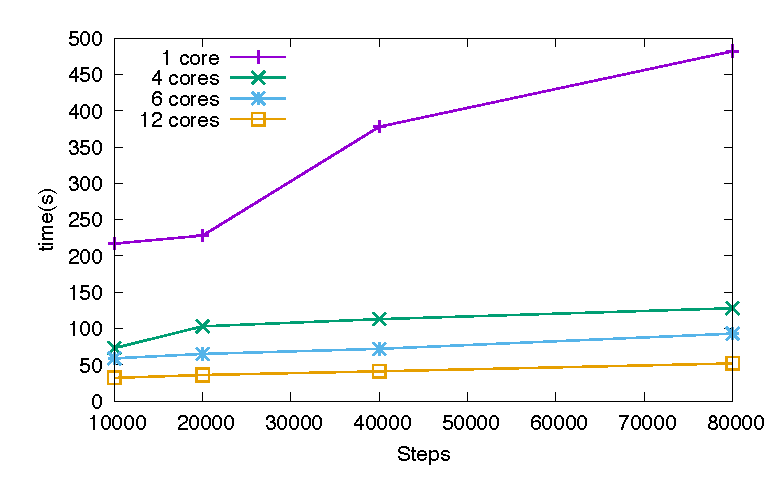
\includegraphics[width=0.95\linewidth]{Chap5/plots/scale.eps}}
\caption[Scalability of KNN2 code on Great Lakes HPC.]{Scalability of KNN2 code for 108,000 atoms on Great Lakes HPC from the University of Michigan with 2x 3.0 GHz Intel Xeon Gold 6154 processors and InfiniBand HDR100 networking, capable of 100 Gb/s throughput.}
\label{Chap:Al/Vac:fig:scale}
\end{figure}
\endgroup


\subsection{\acf{LSKMC}}
\label{Chap:Al/Vac:sec:LSKMC}
One effort we tried to make \ac{kMC} simulation faster is to boost low-energy barrier events by using \acf{LSKMC} invented by Fichthorn et al\cite{fichthorn2013local}. The algorithm goes as shown in Algorithm \ref{algo:lskmc}. Even though the initial and final states of the vacancy are not next to each other in \ac{LSKMC} steps, the corresponding energy change can also be calculated based on a \ac{DFS} method. Because if the \ac{NN} function to predict the barrier is accurate enough, the energy differences along any path the vacancy takes from the initial site to the final site will be the same. We can do \ac{DFS} to look for an available path and use the energy changes along the way to get the energy change between two states. However, the additional computational overhead is inevitable in this method as super-basin states require enumerating methods to explore.

\begin{figure}[!htb]
  \centering
  \begin{minipage}{.75\linewidth}
    \begin{algorithm}[H]
      \caption{\acf{LSKMC} Algorithm from  Fichthorn's method \cite{fichthorn2013local}}\label{algo:lskmc}
      \begin{algorithmic}[1]
        \State set $epoch = 0$, $step = 0$, $time = 0$
        \While{$epoch < epoch_{Max}$}
        \State {perform a regular \ac{kMC} step, get time increment $t$.}
        \State {$time$ += $t$}
        \If{$t < t_{critical}$}
            \State {$step$ += 1}
        \Else
            \State {$step = 0$}
        \EndIf
        \If{$step == step_{critical}$}
            \State {A new super-basin is found.}
            \State {find transient and absorbing states based on preset $E_{critical}$.}
            \State {compute the escape time $t_{escape}$ and probability.}
            \State {decide the exiting state.}
            \State {$time$ += $t_{escape}$}
            \State {$step = 0$}
        \EndIf

        \EndWhile
      \end{algorithmic}
    \end{algorithm}
  \end{minipage}
\end{figure}


Based on the description in Algorithm \ref{algo:lskmc}, there are mainly two hyperparameters, $step_{critical}$ and $E_{critical}$. $step_{critical}$ means after these many steps, we have to involve a local ``super-basin'' step. And $E_{critical}$ is the energy cutoff we set to distinguish transient and absorbing states. If $E < E_{critical}$, then it is a transient state, and the vacancy does not end up in this state afterward. Otherwise, it is an absorbing state. We tested the effects of these two hyperparameters in Figure \ref{Chap:Al/Vac:fig:lskmc_time}. As can be seen, when $step_{critical}$ were set very small and $E_{critical}$ were set very high, many local super-basin steps would be included, and the vacancy is pushed relatively farther away from the trapping sites. There was almost no flat area can be seen in the light blue line. This setup was a high slackness case. On the other hand, when $step_{critical}$ were set very large, and $E_{critical}$ were set very low, yellow or black line, less local super-basin steps are involved, and the vacancy is not pushed very far away. This was a low slackness case. When intermediate values were chosen, the \ac{LSKMC} simulation behaves like regular \ac{kMC} simulations, but needs much fewer steps to achieve the same simulated time and do not stick in low-energy barriers.  Structures and concentrations of generated clusters were also compared to confirm \ac{LSKMC} algorithm does not introduce new stochastic to the simulation results.

\begingroup
\begin{figure}[!ht]
  \centering
  \subfigure{\includegraphics[width=0.95\linewidth]{Chap5/plots/compare_time.pdf}}
\caption[Comparison of different \acf{LSKMC} parameters setup.]{Comparison of different \ac{LSKMC} parameters setup. The x axis shows the number of simulation steps, and the y axis show the corresponding evolution time of the investigated system. In the legend, ``regular'' means the regular \ac{kMC} simulation without any local super-basin steps involved. Other than the ``regular'' label, the first and second numbers in each row of the figure legend correspond to the step count criteria $step_{critical}$ and energy criteria $E_{critical}$, respectively.}
\label{Chap:Al/Vac:fig:lskmc_time}
\end{figure}
\endgroup


\subsection{\acf{LRU} Cache}
\label{Chap:Al/Vac:sec:LRU}
In order to further speed up \ac{kMC} simulations, a \acf{LRU} cache, which evicts the least recently used entry, was implemented based on a hashmap and a  doubly-linked list. The idea is based on memorizing the most recent entries. In this way, if the simulation was stuck in a local minimum, the repeated calculations can be ignored and directly obtained from memory. A similar idea was practiced by Mason et al.\cite{mason2005fast}. They used the ``Zobrist'' key to distinguish different binary alloy cluster structures. However, this method ignored detail local environment differences. Instead, we use the 27-digits encoding and store them in an array as the key. The hashmap holds the keys and the address of the nodes of the doubly-linked list. Each node of the doubly-linked list holds the value of the key, which represents the corresponding vacancy migration barrier. We remove elements from the bottom of the doubly-linked list and add new elements on top of the bottom of the doubly-linked list. When a new entry is accessed, it is moved to the top again, therefore most recently used entries are always on the top, and the least used ones are at the bottom of the list. However, by now, this implementation only supports single-core calculations. To make \ac{LRU} Cache available for multiple cores, one way is to sync or share several most recent entries every several thousands of numbers of steps.

\begingroup
\begin{figure}[!ht]
  \centering
  \subfigure{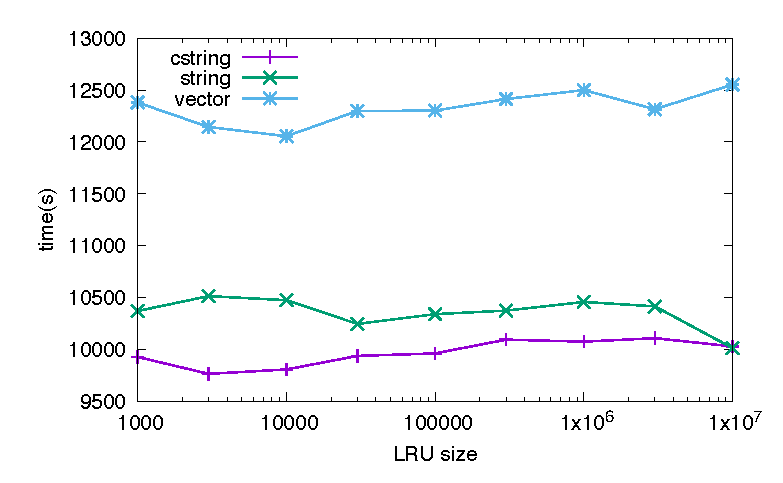
\includegraphics[width=0.95\linewidth]{Chap5/plots/lru_size.eps}}
\caption[Comparison of \acs{LRU} cache size effects on simulation speed for a 108,000-atom supercell system running 10,000,000 steps on TACC Stampede2 cluster.]{Comparison of \acs{LRU} cache size effects on simulation speed for a 108,000-atom supercell system running 10,000,000 steps on TACC Stampede2 cluster. Without using \ac{LRU} cache to memory recent encoding entries, it will take 55,135 seconds to run the simulation.}
\label{Chap:Al/Vac:fig:lru_size}
\end{figure}
\endgroup


To hash on the key of encoding, we tried three different methods: 1) Hashing on a ``long long'' integer. The ``long long'' int data type of C++ for a 64-bit machine can store $2^{64} \sim 1\times10^{19}$ information. 27-digits encoding scheme with Al, Mg, Zn, and Vac can take up to $4^{27} \sim 1\times10^{16}$. Therefore, we can simply convert an encoding array to a decimal integer and hash on the decimal integer. 2) Hashing on a string of C++. 3) Hashing on a C string, which is explicitly an array of char. It turned out that the best strategy would be the third one, directly hashing on a C string in C++ and the best size of \ac{LRU} cache is between 3,000 and 10,000, as shown in Figure \ref{Chap:Al/Vac:fig:lru_size}. Without using \ac{LRU} cache to memory recent encoding entries, it takes 55,135 seconds to run the simulation. In general, the \ac{LRU} cache method provides a 5 times speed-up. Generally speaking, in all the three methods, the speed initially drops and then increases slightly as we increase the size of the \ac{LRU} cache storage capability. This can be explained by the size of the local minimum states. If the \ac{LRU} cache size increase, it also takes a longer time to find the key and may also need more useless insertion operations to the cache.

\begingroup
\begin{figure}[!ht]
  \centering
  \subfigure[]{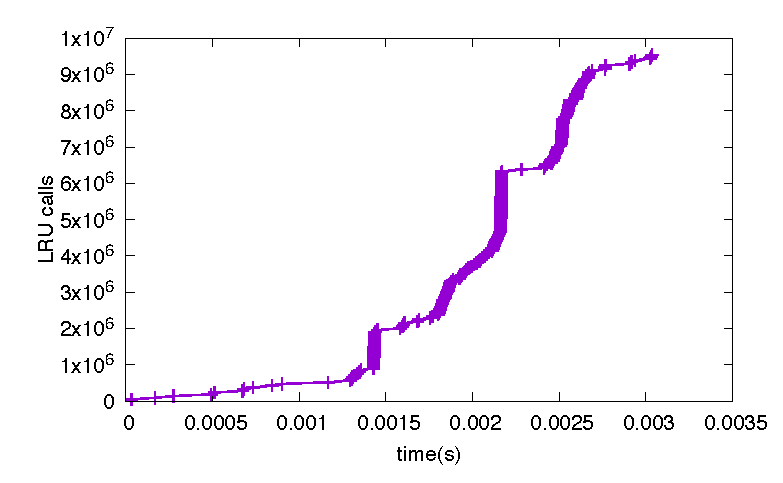
\includegraphics[width=0.85\linewidth]{Chap5/plots/lru_evoke.eps}}\label{Chap:Al/Vac:fig:lru_calls:a}
  \subfigure[]{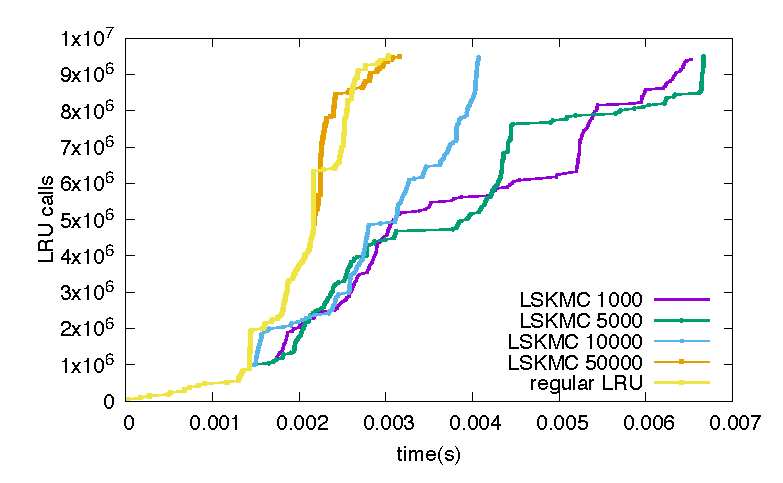
\includegraphics[width=0.85\linewidth]{Chap5/plots/lru_evoke_compare.eps}}\label{Chap:Al/Vac:fig:lru_calls:b}
\caption[Number of calls of \ac{LRU} cached results as time increases.]{Number of calls of \ac{LRU} cached results as time increases. A 3000-entries of \ac{LRU} cache is used. (a) A single-core \ac{LRU} cache for 10,000,000 steps. (b) Comparison of \ac{LRU} with regular \ac{kMC} and \ac{LSKMC} of different local super-basin step involving criteria. Numbers in the legend indicates the value of $step_{critical}$. $E_{critical}$ was chosen to $0.3$ eV for all \ac{LSKMC} simulations in this plot.}
\label{Chap:Al/Vac:fig:lru_calls}
\end{figure}
\endgroup


In Figure \ref{Chap:Al/Vac:fig:lru_calls} (a), we plot the number of \ac{LRU} calls against the simulated time. Initially or during the early stage of simulation, only limited calls happened. Then the number of calls increase significantly around 0.0015, 0.00225, and 0.0025 seconds. This indicates the existence of possible local trapping states. Around these timestamps, the encoding entries stored in the cache have a higher probability of being called. Once the system jumps out of the current low-energy barriers, the number of \ac{LRU} calls becomes sparse again. In Figure \ref{Chap:Al/Vac:fig:lru_calls} (b), we also tested \ac{LRU} cache strategy together with \ac{LSKMC} method. We chose a universal $E_{critical}$ of $0.3$ eV and explored different $step_{critical}$ settings from 1,000 to 50,000. As can be seen from the plot, with very high $step_{critical}$, \ac{LRU} calls invoked just like a regular \ac{kMC}. But when we gradually tune this number lower, the curve becomes less steep and more stair-like. That can be explained by the fact that when \ac{LSKMC} helps the vacancy getting out of the trapped state, less repeating visits happen. Interestingly, for a fixed number of simulation steps, even though with \ac{LSKMC}, a much longer time is achieved, the number of \ac{LRU} calls is on the same order ($1\times10^7$). This is because \ac{LRU} call happens when the event list is built but not during the moment when an event is executed.

